% Created 2019-04-02 Tue 11:50
% Intended LaTeX compiler: pdflatex
\documentclass[a4paper, 12pt]{article}
\usepackage[utf8]{inputenc}
\usepackage[T1]{fontenc}
\usepackage{graphicx}
\usepackage{grffile}
\usepackage{longtable}
\usepackage{wrapfig}
\usepackage{rotating}
\usepackage[normalem]{ulem}
\usepackage{amsmath}
\usepackage{textcomp}
\usepackage{amssymb}
\usepackage{capt-of}
\usepackage{hyperref}
\usepackage[left=2.5cm, right=2.5cm, top=2.5cm, bottom=2.5cm, bindingoffset=1.5cm, head=15pt]{geometry}
\usepackage{setspace}
\usepackage{caption}
\onehalfspacing
\usepackage[official]{eurosym}
\usepackage{amsmath}
\usepackage{amssymb}
\usepackage{notation/rl}
\usepackage{notation/model}
\usepackage{template/list}
\let\itemize\hitemize
\usepackage{fancyhdr}
\pagestyle{fancy}
\fancyhead{}
\fancyfoot{}
\fancyhead[LE,RO]{\textsl{\leftmark}}
\fancyhead[RE,LO]{Tobias Richter}
\fancyfoot[C]{\thepage}
\renewcommand{\headrulewidth}{0.4pt}
\renewcommand{\footrulewidth}{0pt}
\usepackage{apacite}
\let\cite\shortcite
\let\textcite\shortciteA
\usepackage[nohyperlinks]{acronym}
\interfootnotelinepenalty=10000
\usepackage[notlof,notlot,nottoc]{tocbibind}
\newcommand{\studentID}{558305}
\newcommand{\thesistype}{Master Thesis}
\newcommand{\supervisor}{Univ.-Prof. Dr. Wolfgang Ketter}
\newcommand{\cosupervisor}{Karsten Schroer}
\pagenumbering{Roman}
\author{Tobias Richter}
\date{\today}
\title{Reinforcement Learning Portfolio Optimization of Electric Vehicle Virtual Power Plants}
\hypersetup{
 pdfauthor={Tobias Richter},
 pdftitle={Reinforcement Learning Portfolio Optimization of Electric Vehicle Virtual Power Plants},
 pdfkeywords={},
 pdfsubject={},
 pdfcreator={Emacs 26.1 (Org mode 9.2.1)},
 pdflang={English}}
\begin{document}

\makeatletter
\begin{titlepage}
    \begin{center}
        \vspace*{1cm}

        \Large
        \textbf{\@title{}}

        \vspace{1.5cm}

        \thesistype{}

        \vspace{1cm}

        \begin{figure}[htbp]
             \centering
             
\includegraphics[width=.5\linewidth]{./fig/UoC_Logo.png}
        \end{figure}

        \vspace{1cm}

        \large
        \textbf{Author}: \@author{} (Student ID: \studentID{})\\
        \large
        \textbf{Supervisor}: \supervisor{}\\
        \large
        \textbf{Co-Supervisor}: \cosupervisor{}

        \vspace{1cm}
        \large
        Department of Information Systems for Sustainable Society\\
        Faculty of Management, Economics and Social Sciences\\
        University of Cologne\\

        \vspace{1cm}
        \@date{}

    \end{center}
\end{titlepage}
\makeatother
\clearpage
\thispagestyle{empty}
\section*{Eidesstattliche Versicherung}
\label{sec:SOOA}

\vspace{2.5cm}

% Statement of original authorship - Needs to be in German
% see also here: https://www.wiso.uni-koeln.de/sites/fakultaet/dokumente/PA/formulare/eidesstattliche_erklaerung.pdf

Hiermit versichere ich an Eides statt, dass ich die vorliegende Arbeit selbstständig und ohne die Benutzung anderer als der angegebenen Hilfsmittel angefertigt habe. Alle Stellen, die wörtlich oder sinngemäß aus veröffentlichten und nicht veröffentlichten Schriften entnommen wurden, sind als solche kenntlich gemacht. Die Arbeit ist in gleicher oder ähnlicher Form oder auszugsweise im Rahmen einer anderen Prüfung noch nicht vorgelegt worden. Ich versichere, dass die eingereichte elektronische Fassung der eingereichten Druckfassung vollständig entspricht.

\vspace{1cm}

\noindent
Die Strafbarkeit einer falschen eidesstattlichen Versicherung ist mir bekannt, namentlich die Strafandrohung gemäß § 156 StGB bis zu drei Jahren Freiheitsstrafe oder Geldstrafe bei vorsätzlicher Begehung der Tat bzw. gemäß § 161 Abs. 1 StGB bis zu einem Jahr Freiheitsstrafe oder Geldstrafe bei fahrlässiger Begehung.

\vspace{3cm}
\noindent
\textbf{Tobias Richter}

\vspace{0.5cm}
\noindent
Köln, den 01.05.2019
\clearpage

\setcounter{page}{1}
\tableofcontents
\clearpage
\listoffigures
\clearpage
\listoftables
\clearpage

\section*{List of Abbreviations} \markboth{LIST OF ABBREVIATIONS}{}
\begin{acronym}[GCRM]
	\acro{ANN}{Artificial Neural Network}
	\acro{DP}{Dynamic Programming}
	\acro{DSO}{Distribution System Operator}
	\acro{DDQN}{Double Deep Q-Networks}
	\acro{EPEX}{European Power Exchange}
	\acro{EV}{Electric Vehicle}
	\acro{GCRM}{German Control Reserve Market}
	\acro{GP}{Genetic Programming}
	\acro{MAW}{Mean Asymmetric Weighted Objective Function}
	\acro{MC}{Monte Carlo}
	\acro{ML}{Machine Learning}
	\acro{MDP}{Markov Decision Process}
	\acro{PDF}{Probability Density Function}
	\acro{RES}{Renewable Energy Sources}
	\acro{RL}{Reinforcement Learning}
	\acro{TD}{Temporal-Difference}
	\acro{TSO}{Transmission System Operator}
	\acro{V2G}{Vehicle-to-Grid}
	\acro{VPP}{Virtual Power Plant}
\end{acronym}
\clearpage
\section*{Summary of Notation} \markboth{SUMMARY OF NOTATION}{}
Capital letters are used for random variables, whereas lower case letters are used for
the values of random variables and for scalar functions. Quantities that are required to
be real-valued vectors are written in bold and in lower case (even if random variables).
\begin{tabbing}
    \=~~~~~~~~~~~~~~~~~~  \= \kill
    \>$\defeq$            \> equality relationship that is true by definition\\
    \>$\approx$           \> approximately equal\\
    \>$\E{X}$             \> expectation of a random variable $X$, i.e., $\E{X}\defeq\sum_x p(x)x$\\
    \>$\Re$               \> set of real numbers\\
    \>$\leftarrow$        \> assignment\\
    \\
    \>$\e$                \> probability of taking a random action in an \e-greedy policy\\
    \>$\alpha$            \> step-size parameter\\
    \>$\gamma$            \> discount-rate parameter\\
    \>$\lambda$           \> decay-rate parameter for eligibility traces\\
    \\
    \>$s, s'$             \> states\\
    \>$a$                 \> an action\\
    \>$r$                 \> a reward\\
    \>$\S$                \> set of all nonterminal states\\
    \>$\A$                \> set of all available actions\\
    \>$\R$                \> set of all possible rewards, a finite subset of $\Re$\\
    \>$\subset$           \> subset of; e.g., $\R\subset\Re$\\
    \>$\in$               \> is an element of; e.g., $s\in\S$, $r\in\R$\\
    \\
    \>$t$                 \> discrete time step\\
    \>$T, T(t)$           \> final time step of an episode, or of the episode including time step $t$\\
    \>$A_t$               \> action at time $t$\\
    \>$S_t$               \> state at time $t$, typically due, stochastically, to $S_{t-1}$ and $A_{t-1}$\\
    \>$R_t$               \> reward at time $t$, typically due, stochastically, to $S_{t-1}$ and $A_{t-1}$\\
    \>$\pi$               \> policy (decision-making rule)\\
    \>$\pi(s)$            \> action taken in state $s$ under {\it deterministic\/} policy $\pi$\\
    \>$\pi(a|s)$          \> probability of taking action $a$ in state $s$ under {\it stochastic\/} policy $\pi$\\
    \>$G_t$               \> return following time $t$\\
    \\
    \>$\p(s',r|s,a)$      \> probability of transition to state $s'$ with reward $r$, from state $s$ and action $a$\\
    \>$\p(s'|s,a)$        \> probability of transition to state $s'$, from state $s$ taking action $a$\\
    \>$\vpi(s)$           \> value of state $s$ under policy $\pi$ (expected return)\\
    \>$\vstar(s)$         \> value of state $s$ under the optimal policy\\
    \>$\qpi(s,a)$         \> value of taking action $a$ in state $s$ under policy $\pi$\\
    \>$\qstar(s,a)$       \> value of taking action $a$ in state $s$ under the optimal policy\\
    \>$V, V_t$            \> array estimates of state-value function $\vpi$ or $\vstar$\\
    \>$Q, Q_t$            \> array estimates of action-value function $\qpi$ or $\qstar$\\
    \\
    \>$d$                 \> dimensionality---the number of components of $\w$\\
    \>$\w$                \> $d$-vector of weights underlying an approximate value function\\
    \>$\hat v(s,\w)$      \> approximate value of state $s$ given weight vector $\w$\\
    \>$\mu(s)$            \> on-policy distribution over states\\
    \>$\MSVEm$            \> mean square value error\\
\end{tabbing}
\clearpage

\pagenumbering{arabic}
\section{Empirical Setting}
\label{sec:org68646b7}
This research is embedded in the German carsharing and electricity markets.
Germany is a suitable testbed, since it has a comparably high share of
renewables in its energy mix and is pushing for an energy turnaround (German:
\emph{Energiewende}) since 2010 \cite{bmu10_energ_concep_envir_sound_reliab_affor}
The high renewable energy content in the energy mix causes electricity prices to
be volatile, which makes Germany an attractive location for the use of
VPPs.

Germany is home to the carsharing providers Car2Go\footnote{\url{https://www.car2go.com}} and DriveNow\footnote{\url{https://www.drive-now.com}},
which operate large EV fleets across the globe. It has been argued that electric
carsharing can simultaneously solve several traditional mobility and
environmental problems and are an important element of future smart cities
\cite{firnkorn15_free_float_elect_carsh_fleet_smart_cities}. Further, it is widely
regarded that the future of mobility will be electric, shared, smart and
eventually autonomous \cite{burns13_sustain_mobil,sterling18_three_revol}.
Carsharing providers are already contributing to the first two points by
operating large fleets of electric vehicles. This research addresses the third
point: Using electric carsharing fleets to smartly participate in electricity
markets. Carsharing providers, like Car2Go and DriveNow, operate their
carsharing fleets in a free-float model, which allows customers to pick up and
drop vehicles at any place within the operating zone of the provider. Customers
pay by the minute and are offered incentives to park the EVs at charging
stations at the end of their trip.

We obtained real-world trip data from Daimler's carsharing service Car2Go.
Additionally, we collected freely available balancing market data from the GCRM
platform website \url{https://regelleistung.net}. The data of the EPEX Spot market
have kindly been provided by ProCom GmbH\footnote{\url{https://procom-energy.de}} for research purposes. In the
next chapters the different datasets are described, as well the most important
processing steps outlined.

\subsection{Electronic Vehicle Fleet Data}
\label{sec:org52ca790}
The Car2Go dataset consists of GPS data of around 500 Smart ED3 Fortwo vehicles in
Stuttgart. These subcompact cars are equipped with a 17.6kWh battery and a
standard 3.3kW on-board charger. They fully charge in about six to seven hours
and can reach a maximum driving distance of 145km according to the manufacturer.
When equipped with an additional 22kW fast charger the charging time reduces to
about an hour.

In Table \ref{table-car2go-raw} the raw data is displayed, as we have obtained it
by Car2Go. The dataset contains spatio-temporal attributes, such as timestamp,
coordinates, and the address of the EVs in 5 minute intervals. Additionally,
status attributes of the interior and exterior are given (not displayed).
Especially relevant for our research is the state of charge (\(SoC\), in \%) and
information whether the EV is plugged into one of the 380 charging stations in
Stuttgart. Note that the data only contain EVs that are \emph{available for rent},
i.e., they are not currently rented out by a customer. EVs which are parked at a
charging station are also not available until they have charged up approximately
70 SoC. Individual trips have to be reconstructed using the GPS data of the
cars. The following preprocessing steps have been taken to prepare the data for
further analysis. Table \ref{table-car2go-processed} depicts the dataset after all
processing steps.

\begin{enumerate}
\item Drop unused data columns

\begin{itemize}
\item \emph{ID}: Number plate is already a unique identifier for every EV.
\item \emph{Address}: Different addresses were given from same coordinates. \emph{Latitude,
Longitude} was used for locational data instead.
\item \emph{Interior, Exterior}: Status attributes were not used in the analysis of
this research. Although they could form interesting features for rental
predictions.
\item \emph{Engine Type}: All EVs in Stuttgart are electric vehicles.
\end{itemize}
\item Decrease GPS resolution to 10 meters

The GPS accuracy of private industry sensors is approximately 5 meters under
open sky, and worse near buildings, bridges and trees\footnote{See \url{https://www.gps.gov/systems/gps/performance/accuracy}, accessed
23\textsuperscript{th} February 2019.}. Rental trips are
identified by changing GPS locations of the EV (See next point). To reduce
the number of false identified trips, due to GPS measurement errors, the resolution
is decreased.
\item Determine rental trips

We infer that a customer rented an EV, if the position coordinates change
between two data points of the same EV (see Table \ref{table-car2go-raw}, 4\textsuperscript{th}
to 5\textsuperscript{th} row). Note that we assume that customer do not undertake trips,
which begin and end at the exact same location.
\item Infer charging stations

The GPS location of the EVs is matched with the GPS locations, where an EV
has been charged at least once in the dataset. We observed that the raw data
do not show EVs that are parked at charging stations, but are not plugged in.
This research assumes that all EVs, which are parked at charging stations are
also plugged in. That is a valid assumption, since in Germany cars are only
allowed to park at charging station if they are connected to it.
\item Clean data
\begin{itemize}
\item \emph{Service trips}: 999 rental trips were removed that had a trip duration
longer than the maximum allowed rental time of two days. We assume that
these trips were \emph{service trips} undertaken by Car2Go. When the EVs
returned with a higher SoC (e.g., they have been charged at the car repair
shop), the previous trip had to be altered to end at a charging station to
ensure charging consistency.
\item \emph{Incorrectly charged EVs}: 999 EVs were removed that show incorrect
charging behavior. The data of these EVs showed an increase of more than
20\% SoC between trips or on trips, while not being located at a charging
station.
\end{itemize}
\end{enumerate}

\begin{sidewaystable}[htbp]
    \caption{Sample Raw Car2Go Data in Stuttgart \label{table-car2go-raw}}
    \centering
    \begin{tabular}{c|ccccccc}
      \hline
      \hline
      Number Plate & Timestamp & Latitude & Longitude & Street & Zip Code & Charging & SoC (\%)\\
      \hline
      S-GO2471 & 24.12.2017 20:00 & 9.19121 & 48.68895 & Parkplatz Flughafen & 70692 & no & 94\\
      S-GO2471 & \ldots{} & \ldots{} & \ldots{} & \ldots{} & \ldots{} & \ldots{}. & \ldots{}\\
      S-GO2471 & 24.12.2017 20:05 & 9.19121 & 48.68895 & Parkplatz Flughafen & 70692 & no & 94\\
      S-GO2471 & 24.12.2017 20:10 & 9.19121 & 48.68895 & Parkplatz Flughafen & 70692 & no & 94\\
      S-GO2471 & 24.12.2017 23:05 & 9.15922 & 48.78848 & Salzmannweg 3 & 70192 & no & 71\\
      S-GO2471 & 24.12.2017 23:10 & 9.15922 & 48.78848 & Salzmannweg 3 & 70192 & no & 71\\
      S-GO2471 & 25.12.2017 00:40 & 9.17496 & 48.74928 & Felix-Dahn-Str. 45 & 70597 & yes & 62\\
      S-GO2471 & 25.12.2017 00:45 & 9.17496 & 48.74928 & Felix-Dahn-Str. 45 & 70597 & yes & 64\\
      S-GO2471 & \ldots{} & \ldots{} & \ldots{} & \ldots{} & \ldots{} & \ldots{}. & \ldots{}\\
      S-GO2471 & 25.12.2017 06:50 & 9.17496 & 48.74928 & Felix-Dahn-Str. 45 & 70597 & no & 100\\
      S-GO2471 & 25.12.2017 08:25 & 9.2167 & 48.78742 & Friedenaustraße 25 & 70188 & no & 42\\
      \hline
      \hline
    \end{tabular}

    \bigskip\bigskip  % provide some separation between the two tables

    \caption{Sample Processed Car2Go Trip Data in Stuttgart \label{table-car2go-processed}}
    \centering
    \begin{tabular}{cc|ccccc}
      \hline
      \hline
      Number Plate & Trip & Start Time & Start Latitude & Start Longitude & Start SoC (\%)\\
      \hline
      S-GO2471 & 1 & 24.12.2017 20:10 & 9.19121 & 48.6890 & 94\\
      S-GO2471 & 2 & 24.12.2017 23:10 & 9.15922 & 48.7885 & 71\\
      S-GO2471 & 3 & 25.12.2017 06:50 & 9.17496 & 48.7493 & 66\\
      \hline
      Number Plate & Trip & End Time & End Latitude & End Longitude & End SoC (\%)\\
      \hline
      S-GO2471 & 1 & 24.12.2017 23:05 & 9.15922 & 48.7885 & 71\\
      S-GO2471 & 2 & 25.12.2017 00:40 & 9.17496 & 48.7493 & 62\\
      S-GO2471 & 3 & 25.12.2017 08:25 & 9.2167 & 48.7875 & 42\\
      \hline
      Number Plate & Trip & Trip Duration (min) & Trip Distance (km) & Trip Charge (\%) & End Charging\\
      \hline
      S-GO2471 & 1 & 175 & 33.35 & 23 & no\\
      S-GO2471 & 2 & 90 & 13.05 & 9 & yes\\
      S-GO2471 & 3 & 155 & 29 & 20 & no\\
      \hline
      \hline
    \end{tabular}
\end{sidewaystable}

\subsection{Balancing Market Data \label{sec-data-balancing}}
\label{sec:org6b6d87f}
In this research, we use market balancing data from the German secondary reserve
market. The following chapter will give an overview of the dataset and
preprocessing steps that were taken. The data encompasses weekly lists of
anonymized bids between 01.06.2016 and 01.01.2018 and a dataset of activated
control reserve in Germany during the same period. For a detailed description
about the market design of balancing markets refer to Chapter
\ref{sec-balancing-market}.

The bidding data consists of the traded electricity product, the offered
capacity \(\Pb{}\) (MW), the capacity price \(\cp{}\) (\(\emw\)), and the
energy price \(\ep{}\) (\(\emwh\)) of each bid. Four different products
are traded, which are a combination of positive control reserve (feed
electricity into the grid) or negative control reserve (take electricity from
the grid) and the provided time segment (peak or non-peak hours). Since negative
prices are allowed on the secondary operating reserve market, the payment
direction is included as well. Moreover, information about the amount of
capacity that was accepted, i.e., either partially or fully, is listed. Bids,
which were not accepted by the TSOs are not listed. An exemplary excerpt of the
dataset is displayed in Table \ref{table-operating-reserve}.

\begin{longtable}{c|ccccc}
\caption[Secondary Operating Reserve Market Data]{List of Bids of the German Secondary Reserve Market for the tender period 04.12.2017 - 11.12.2017. \label{table-operating-reserve}}
\\
\hline
\hline
Product & Capacity Price & Energy Price & Payment & Offered & Accepted\\
\hline
\endfirsthead
\multicolumn{6}{l}{Continued from previous page} \\
\hline

Product & Capacity Price & Energy Price & Payment & Offered & Accepted \\

\hline
\endhead
\hline\multicolumn{6}{r}{Continued on next page} \\
\endfoot
\endlastfoot
\hline
NEG-HT & 0 & 1.1 & TSO to bidder & 5 & 5\\
NEG-HT & 10.73 & 251 & TSO to bidder & 15 & 15\\
NEG-HT & 200.3 & 564 & TSO to bidder & 22 & 22\\
\ldots{} & \ldots{} & \ldots{} & \ldots{} & \ldots{} & \ldots{}\\
NEG-NT & 0 & 21.9 & Bidder to TSO & 5 & 5\\
NEG-NT & 0 & 22.4 & Bidder to TSO & 5 & 5\\
\ldots{} & \ldots{} & \ldots{} & \ldots{} & \ldots{} & \ldots{}\\
POS-NT & 696.6 & 1200 & TSO to bidder & 5 & 5\\
POS-NT & 717.12 & 1210 & TSO to bidder & 10 & 7\\
\hline
\hline
\end{longtable}

In this study, we assume that bidding on 15-minute intervals in secondary
operating reserve auctions will be possible in future energy markets. As
mentioned in Chapter \ref{sec-balancing-market}, the market design of the GCRM
secondary operating reserve tender was adjusted in 2017. Daily tenders with
4-hour bidding intervals were introduced in favor of weekly tenders with only
two time segments. This change represents the trend by the TSOs to change the
market design in order to better include RES into the operating reserve markets
\cite{agricola14_dena_ancil_servic_study}. Due to the volatility of renewable
electricity generation, providers are naturally dependent on accurate short-term
forecasts, which are only possible with short tender periods and fine-grained
bidding intervals.

In order to estimate the upper bound of profits that the EV fleet can earn by
participating in the secondary operating reserve market, the \emph{critical prices}
\(\ccp{}\) and \(\cep{}\) were determined for each auctioned interval. Following
\textcite{brandt17_evaluat_busin_model_vehic_grid_integ}, we define \(\ccp{}\)
(\(\emw\)) as the capacity price of the bid that was just barely
accepted, whereas \(\cep{}\) (\(\emwh\)) is the highest energy price
that was payed for activated control reserve during that interval. For every
15-minute interval within the given tender period of one week, the activated
control reserve in that interval was matched with the accepted bids in that
tender period. At the point where supply, i.e., offered capacity of bids, met
demand, i.e., activated control reserve, the critical price \(\cep{}\) was
determined.

\emph{Example}: The assumed critical prices for the secondary operating reserve
tender interval of the 6\textsuperscript{th} December 2017 between 08:00 and 08:15 are obtained
as follows: Three suppliers submitted a reserve capacity of 5MW, 15MW and 22MW
respectively (see Table \ref{table-operating-reserve}). The critical capacity
price \(\ccp{}\!=\!200.3\emw\) is determined by the capacity price of the last
(third) accepted bid in that time segment. The TSO reported that 18MW of control
reserve were activated between 08:00 and 08:15. Hence, the second bid determines
the critical energy price \(\cep{}\!=\!251\emwh\), as control reserve capacity
gets activated according to ascending order of the submitted energy prices. In
this example the second bidder would get compensated with:
\(R\!=\!R^c + R^e\!=\!(10.73\emw\!\times\!15\mw) +
(251\emwh\!\times13\mw\!\times\!0.25\text{h})\!=\! 976.7\eur\). Note that
the second bidder get compensated for providing 13MW for 15 minutes (0.25h),
instead of the submitted 15MW, since in total only 18MW of control capacity was
activated, which was partly fulfilled by the 5MW of the first bidder.

\subsection{Spot Market Data \label{sec-data-intraday}}
\label{sec:org648dc59}
The data from the EPEX Spot Intraday Continuous encompass order books and
executed trades from 01.06.2016 until 01.01.2018. The list of trades contain
information on the unit price \(\up{}\) (\(\emwh\)), the quantity (kW)
and the traded product (hourly, quarterly or block). In this research, we focus
on quarterly product times (15-minute intervals), as they provide the highest
flexibility. Fleet controllers can promptly react to fluctuant electricity
demand of the EV fleet by accurately adjusting the bid quantities. Future
research could also consider other electricity products if lower prices justify
decreased flexibility at that point in time. Additionally, the TSOs of the buyer
and seller are listed in the dataset. They are only relevant if special
conditions between TSO apply, e.g., when delivering electricity to other
countries.

On the spot market, electricity trades can have a very short lead time of up to
5 minutes before delivery (see Table \ref{table-spot-market}). This market
characteristic is beneficial for our proposed trading strategy, since it allows
the EV to procure electricity in almost real time. The controller can submit
bids to the market, with accurate estimations of available charging capacity up
to five minutes ahead. Similarly to the balancing market, the critical price
\(\cup{}\) has to be determined for all intraday trading intervals. The critical
unit price \(\cup{}\) is defined as the lowest price of all executed trades.
\begin{equation*}
    \cup{} \defeq \min_{t \in \cal{T}} \up{t} \text{ ,}
\end{equation*}
where \(\cal{T}\) is the set of all trades in a bidding interval. \emph{Example:} The
critical unit price of the trades in Table \ref{table-spot-market} is \(\cup{}
\!=\!51.00 \emwh\) (trades 8031392, 8031387 and 8031375). All buyers that submitted
bids with a price higher than the critical unit price, successfully procured
electricity. Hence, accurate forecasts of the critical price allow to optimize the
bidding behavior. For a detailed description of the intraday continuous market
see Chapter \ref{sec-spot-market}.

{\captionsetup[table]{aboveskip=0.5cm}
\begin{sidewaystable}[hp]
\caption{List of Trades of the EPEX Spot Intraday Continuous Market \label{table-spot-market}}
\centering
\begin{tabular}{c|cccccccc}
\hline
\hline
Execution time & ID & Unit Price & Quantity & Buyer Area & Seller Area & Product & Product Time & Delivery Date\\
\hline
2017-12-04 06:54:55 & 8031392 & 51.00 & 5500 & Amprion & Amprion & Quarter & 07:15 - 07:30 & 2017-12-04\\
2017-12-04 06:53:26 & 8031391 & 59.00 & 10000 & TenneT & TenneT & Quarter & 07:15 - 07:30 & 2017-12-04\\
2017-12-04 06:53:26 & 8031390 & 58.90 & 10000 & TenneT & TenneT & Quarter & 07:15 - 07:30 & 2017-12-04\\
2017-12-04 06:53:15 & 8031389 & 52.30 & 7000 & 50Hertz & 50Hertz & Quarter & 07:15 - 07:30 & 2017-12-04\\
2017-12-04 06:53:13 & 8031386 & 59.00 & 500 & TenneT & TenneT & Quarter & 07:15 - 07:30 & 2017-12-04\\
2017-12-04 06:53:13 & 8031387 & 51.00 & 3600 & Amprion & Amprion & Quarter & 07:15 - 07:30 & 2017-12-04\\
2017-12-04 06:53:13 & 8031388 & 52.00 & 1400 & Amprion & Amprion & Quarter & 07:15 - 07:30 & 2017-12-04\\
2017-12-04 06:53:02 & 8031385 & 58.90 & 11000 & TenneT & TenneT & Quarter & 07:15 - 07:30 & 2017-12-04\\
2017-12-04 06:52:38 & 8031380 & 60.00 & 10000 & Amprion & Amprion & Quarter & 07:15 - 07:30 & 2017-12-04\\
2017-12-04 06:52:38 & 8031381 & 57.50 & 8000 & Amprion & Amprion & Quarter & 07:15 - 07:30 & 2017-12-04\\
2017-12-04 06:52:38 & 8031382 & 58.00 & 2000 & Amprion & Amprion & Quarter & 07:15 - 07:30 & 2017-12-04\\
2017-12-04 06:52:38 & 8031383 & 58.90 & 4000 & TenneT & TenneT & Quarter & 07:15 - 07:30 & 2017-12-04\\
2017-12-04 06:52:38 & 8031384 & 60.00 & 4000 & Amprion & Amprion & Quarter & 07:15 - 07:30 & 2017-12-04\\
2017-12-04 06:52:27 & 8031379 & 52.30 & 8000 & 50Hertz & 50Hertz & Quarter & 07:15 - 07:30 & 2017-12-04\\
2017-12-04 06:51:33 & 8031378 & 66.00 & 5000 & TransnetBW & TransnetBW & Quarter & 07:15 - 07:30 & 2017-12-04\\
2017-12-04 06:51:28 & 8031377 & 54.00 & 8000 & Amprion & Amprion & Quarter & 07:15 - 07:30 & 2017-12-04\\
2017-12-04 06:51:24 & 8031376 & 54.00 & 7000 & TenneT & TenneT & Quarter & 07:15 - 07:30 & 2017-12-04\\
2017-12-04 06:49:34 & 8031375 & 51.00 & 4000 & TenneT & TenneT & Quarter & 07:15 - 07:30 & 2017-12-04\\
2017-12-04 06:49:26 & 8031374 & 54.00 & 5000 & 50Hertz & 50Hertz & Quarter & 07:15 - 07:30 & 2017-12-04\\
2017-12-04 06:49:23 & 8031373 & 55.10 & 8000 & 50Hertz & 50Hertz & Quarter & 07:15 - 07:30 & 2017-12-04\\
\hline
\hline
\end{tabular}
\end{sidewaystable}
}

\clearpage

\section{Model}
\label{sec:org6031556}
The following chapter will introduce the model of this research. In its essence,
we propose a solution for EV fleet providers to utilize a VPP portfolio to
profitably provide balancing services to the grid on multiple markets. A control
mechanism procures energy from electricity markets, allocates available EVs to
VPPs, and intelligently dispatches EVs to charge the acquired amount of energy.
The model employs a RL agent that learns an optimal bidding strategy by
interacting with the electricity markets and reacts to changing rental demand of
the EV fleet. This chapter is structured as follows: The information assumptions
are listed first, the control mechanism is explained next, and finally, the RL
approach is described in detail. The used notation in this chapter can be found
in Table \ref{table-notation}.

We formulate the problem as a \emph{controlled EV charging} problem. The EV fleet
operator represents the \emph{controller}, which aims to charge the fleet at minimal
costs. First, the controller predicts the amount of energy it can charge in a
given \emph{market period} \(h\). The length of the market period \(\Delta h\) and the
market closing time depend on the considered electricity market. Second, the
controller places bids on one or multiple markets to procure the predicted
amount of energy. Lastly, at electricity delivery time, the controller
communicates with the EV fleet to control the charging in real-time. Online EV
\emph{control periods} \(t\) are typically shorter than market periods. In the
empirical case that we consider, the market periods are 15 minutes long, while
the EV control periods last 5 minutes. Nonetheless, the presented approach
generalizes to other period lengths. During each control period, the controller
has to take decisions which individual EVs it should dispatch to charge the
procured amount of electricity. In times of unforeseen rental demand, this
decision implies trading off commitments to the markets with compromising
customer mobility by refusing customer rentals.


\begin{longtable}{p{0.11\linewidth}|p{0.75\linewidth}|c}
\caption[Table of Notation]{Table of Notation \label{table-notation}}
\\
\hline
\hline
Symbol & Description & Unit\\
\hline
\endfirsthead
\multicolumn{3}{l}{Continued from previous page} \\
\hline

Symbol & Description & Unit \\

\hline
\endhead
\hline\multicolumn{3}{r}{Continued on next page} \\
\endfoot
\endlastfoot
\hline
\(t\) & Control period. & -\\
\(h\) & Market period. & -\\
\(T\) & Number of control periods in a market period. & -\\
\(H\) & Number of market periods in day. & -\\
\(N_h\) & Total number of market periods. & -\\
\(\Delta t\) & Length of control period. & hours\\
\(\Delta h\) & Length of market period. & hours\\
\hline
\(\Pb{h}\) & Amount of balancing power offered on the balancing market. & kW\\
\(\ccp{h}\) & Critical capacity price in market period \(h\). & \(\emw\)\\
\(\cep{h}\) & Critical energy price in market period \(h\). & \(\emwh\)\\
\(\Pi{h}\) & Amount of power offered for the unit on the intraday market. & kW\\
\(\cup{h}\) & Critical unit price in market period \(h\). & \(\emwh\)\\
\(\Eb{h}\) & Amount of energy charged from balancing market in market period h. & MWh\\
\(\Ei{h}\) & Amount of energy charged from the intraday market in market period h. & MWh\\
\hline
\(\fP{t}\) & Amount of available fleet charging power in control period \(t\). & kW\\
\(\fPhat{t}\) & Predicted amount of available fleet charging power in control period \(t\). & kW\\
\hline
\(\Cb{h}(P)\) & Cost function for procuring electricity from the balancing market. & \(\eur\)\\
\(\Ci{h}(P)\) & Cost function for procuring electricity from the intraday market. & \(\eur\)\\
\(\oc\) & Opportunity costs of lost rental of EV \(i\) in control period \(t\). & \(\eur\)\\
\(\beta_h\) & Imbalance costs in market period \(h\). & \(\eur\)\\
\hline
\(\lb{h}\) & Balancing market risk factor. & \([0,1]\)\\
\(\li{h}\) & Intraday market risk factor. & \([0,1]\)\\
\(\theta_{\lambda}\) & Set of risk factors for all market periods \(h\!\in\!\{1,...,N_h\}\). & -\\
\(\Cf{}(\theta_{\lambda})\) & Cost function for the fleets total costs over all market periods \(h\). & \(\eur\)\\
\(\Cf{h}\) & Total accumulated fleet costs until market period \(h\). & \(\eur\)\\
\hline
\(i\) & Electric Vehicle. & -\\
\(\F\) & Set of all EVs in the fleet & -\\
\(\c\) & Dummy variable if EV is connected to a charging station. & 0/1\\
\(\omega_{i}\) & Amount of electricity stored in EV. & \(\kwh\)\\
\(\Omega\) & Maximum battery capacity of EV. & \(\kwh\)\\
\(\delta\) & Charging power of EV at the charging station. & \(\kw\)\\
\(p^{ind}\) & Industry tariff & \(\ekwh\)\\
\hline
\end{longtable}

\subsection{Assumptions \label{sec-model-assumptions}}
\label{sec:orgcc4f254}

In order to evaluate and operationalize our model, the following assumptions
about the available information and the electricity market mechanism are taken:
\subsubsection{Information Assumptions}
\label{sec:org805815f}

\begin{enumerate}
\item Mobility demand

The controller is able to forecast the mobility demand of the EV fleet with
different time-horizons based on historical data. More specifically, it can
predict the amount of plugged-in EVs and consequently the available charging
power \(P^{fleet}_t\) of the fleet at control period \(t\). The prediction
accuracy is increasing with shorter time horizons, from uncertain predictions
one week ahead to very accurate predictions 30 minutes ahead. Past research
presented successful mobility demand forecast algorithms in the context of
free-float carsharing
\cite{kahlen18_elect_vehic_virtual_power_plant_dilem,kahlen17_fleet,wagner16_in_free_float}.
\item Critical electricity prices

The controller is able to forecast electricity prices of spot and balancing
markets based on historical data. More specifically, it can estimate the
critical prices \(\ccp{h}\), \(\cep{h}\), and \(\cup{h}\) for each market period
with perfect accuracy (see Chapter \ref{sec-data-balancing} and Chapter
\ref{sec-data-intraday} for the critical price definitions). Electricity price
forecasting is an extensively studied research area with well-advanced
prediction algorithms
\cite{weron14_elect_price_forec,avci18_manag_elect_price_model_risk}.
\end{enumerate}
We are confident that taking the above assumptions is viable, assuming available
forecasting information is common practice in the VPP and EV fleet charging
literature, for example
\textcite{vandael15_reinf_learn_heuris_ev_fleet,mashhour11_biddin_strat_virtual_power_plant_1,tomic07_using_fleet_elect_drive_vehic_grid_suppor,pandzic13_offer_model_virtual_power_plant}.

\subsubsection{Market Assumptions}
\label{sec:org2955ee2}
\begin{enumerate}
\item Balancing market

The controller is able to submit bids of any quantity for single 15-minute
market periods 7 days ahead. Since the critical capacity and energy prices
are available (previous paragraph), the controller submits bids in the form
\(bid\!=\!(\Pb{},\ccp{},\cep{})\). Submitting a bid with the critical capacity
price ensures that the bid will always get accepted by the TSOs. Submitting
the bid with the critical energy price ensures that the balancing power will
always get fully activated, which allows the fleet to charge at the submitted
price for the market periods length.

\item Intraday market

The controller submits bids to the intraday market 30 minutes ahead. The bids
are submitted in the form \(bid\!=\!(\Pi{},\cup{})\). We assume that the order
to buy will always get matched until the minimal lead time of the trade
(e.g., 5 minutes on the EPEX Spot Intraday Continuous). In reality, this is
not always the case since trades are executed immediately and it is not
guaranteed that a matching order to sell is submitted between the bidding
time and the minimal lead time.
\end{enumerate}
In essence, we are assuming that the controller always submits the optimal bid
at the right time. In other words, every bid leads to the successful procurement
of the desired amount of electricity. This assumption provides an upper bound
for the fleet profits from trading EV battery storage on the electricity
markets. However, the upper bound is only influenced by the accuracy of the
electricity price forecasting algorithm, a research area that well exceeds the
scope of this work. Furthermore, we assume that the controller is a price-taker.
Due to the limited size of its bids, it is lacking the market share to influence
prices on the markets. Similar assumptions have been made by
\textcite{brandt17_evaluat_busin_model_vehic_grid_integ} and
\textcite{vandael15_reinf_learn_heuris_ev_fleet}.
\subsection{Control Mechanism}
\label{sec:orgfcef806}
The control mechanism constitutes the core of this research. It can be seen as a
decision support system that can be deployed at an EV fleet operator to centrally
control the charging of its fleet. Figure \ref{fig-control-mechanism} depicts the
control mechanism, which is divided into three distinct phases:

The first phase, \emph{Bidding Phase I}, takes place just before the closing time of
the balancing market, once every week (e.g., Wednesdays at 3pm at the GCRM). In
this phase, the controller can place bids for every market period \(h\) of the
following week on the balancing market. The second phase, \emph{Bidding Phase II},
takes places in every market period of \(\Delta{h}\!=\!15\) minutes. At this
point, the controller has the opportunity to place bids to the intraday market
for the market period 30 minutes ahead. The third phase, \emph{Dispatch Phase}, takes
places in every control period of \(\Delta{t}\!=\!5\) minutes. In this phase the
controller has to dispatch available EVs to charge the procured electricity from
the markets. The phase involves allocating individual EVs to the VPP and
potentially refusing customer rentals to assure that all market commitments can
be fulfilled.

The following chapters will highlight the important parts of the three phases
and provide detailed explanation and mathematical formulations.

\begin{figure}[p]
\centering
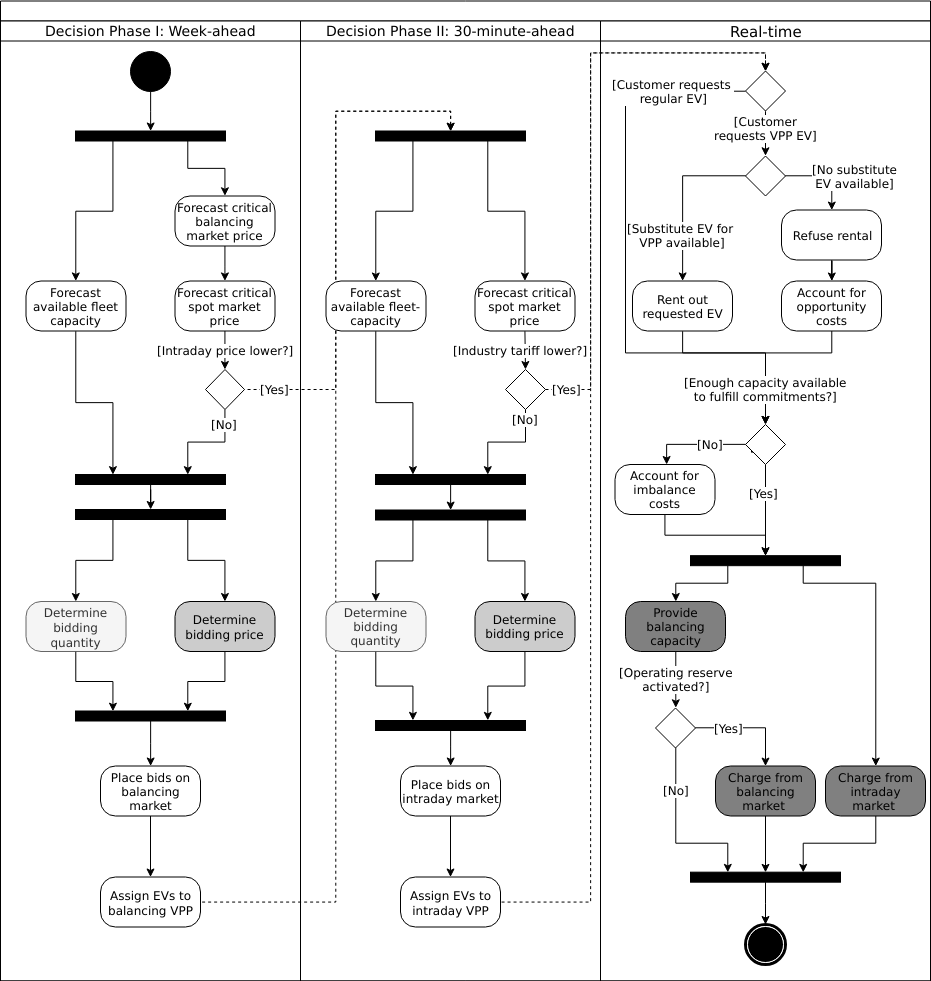
\includegraphics[width=1.05\linewidth]{fig/control_mechanism.png}
\caption[Control Mechanism]{Control Mechanism \label{fig-control-mechanism}}
\end{figure}

\subsubsection{Fleet Charging Power Prediction}
\label{sec:org81e04c7}

In a first step, the controller has to predict the available fleet charging
power for the market period of interest (see\circled{A} in Figure
\ref{fig-control-mechanism}). The actual available fleet charging power \(\fP{t}\)
in a control period \(t\) is given by the number of EVs that are connected to a
charging station, with enough free battery capacity to charge the next control
period \(t\!+\!1\).

When the controller procures electricity from the markets, the fleet has to
charge with the committed charging power during all control periods of the
market period \(h\), otherwise imbalance costs occur. To minimize the risk of not
being able to charge the committed amount of energy during the whole market
period, the predicted fleet charging power in a market period is defined as the
minimal predicted fleet charging power of all control periods in that market
period:
\begin{equation}
    \fPhat{h} \defeq \min_{n \in \{1, .., T\}} \fPhat{t + n} \text{ ,}
\end{equation}
where \(h\) is the market period of interest, \(t\) its first control period and \(T\)
the number of control periods in a market period.



\subsubsection{Market Decision}
\label{sec:orgb72932f}
In a second step, the controller has to decide from which market it should
procure the desired amount of energy (see\circled{B} in Figure
\ref{fig-control-mechanism}). Therefore, it compares the costs for charging
electricity from the balancing market with the costs for charging from the
intraday market. The cost function for procuring electricity from the balancing
market is defined as follows:
\begin{equation} \label{eq-cost-balancing}
\begin{split}
    \Cb{h}(P) &\defeq -(P\!\times\!10^{-3} \times \ccp{h}) + (\Eb{h} \times \cep{h}) \\
    &= -(P\!\times\!10^{-3} \times \ccp{h}) + (P \frac{\Delta h}{10^{3}} \times \cep{h}) \text{ ,}
\end{split}
\end{equation}
where \(P\) (kW) is the amount of offered balancing power. The first term of the
equation corresponds to the compensation the controller retrieves for keeping
the balancing capacity available, while the second term corresponds to the costs
for charging the activated balancing energy \(\Eb{h}\) (MWh). Energy is power over
time, hence \(\Eb{h}\) can be substituted with \(P\) times the market periods length
\(\Delta{h}\), divided by the unit conversion term from kW to MW. Note that the
critical energy price \(\cep{}\!\in\!\Re\), can also take negative values,
resulting in profits for the fleet, while the critical capacity price
\(\ccp{}\!\in\! \Re^+_0\) is never negative and therefore never results in
costs for the fleet.

The cost function for charging from the intraday market is defined similarly to
\eqref{eq-cost-balancing}:
\begin{equation}
\begin{split}
    \Ci{h}(P) &\defeq \Ei{h} \times \cup{h} \\
    &= P \frac{\Delta h}{10^{3}}\times \cup{h}
\end{split}
\end{equation}
Again, depending on the market situation, \(\cup{}\!\in\!\Re\) can either be
negative or positive, resulting in costs or profits for the fleet. Contrarily to
the balancing market, on the intraday market the fleet does not get compensated
for keeping the charging power available; only the charged energy affects the
costs. If the costs for charging from the balancing market 7 days ahead
\(\Cb{h+(7\!\times\!H)}(\fPhat{h+(7\!\times\!H)})\) are higher than the costs of
charging from the intraday market at the same market period \(\Ci{h +
(7\!\times\!H)}(\fPhat{h+(7\!\times\!H)})\), the controller does not procure
electricity from the balancing market.

\subsubsection{Determining the Bidding Quantity}
\label{sec:orgaea6adc}
In a third step, the controller has to take a decision on the amount of energy
it should procure from the markets (see\circled{C} in Figure
\ref{fig-control-mechanism}). Determining the bidding quantity is the core
challenge of the controlled charging problem. The bidding quantity determines
the profits that can be made, by charging at a cheaper market price than the
flat industry tariff. On one hand, the controller aims to maximize its profits
by procuring as much electricity as possible from the markets. On the other
hand, it needs to balance the risk of (a) procuring more energy that it can
maximally charge and (b) not procuring enough energy from the market to
sufficiently charge the fleet.

In case (a), the fleet is facing costs of compromising customer mobility, or
worse, high imbalance penalties from the markets. Renting out EVs is
considerably more profitable than using their batteries as a VPP. Refusing
customer rentals, in order to fulfill market commitments, induces opportunity
costs of lost rentals \(\rho\) on the fleet. Imbalance costs \(\beta\) occur, when
the fleet can not charge the committed amount energy at all, even with refusing
rentals. In case (b), the fleet also faces opportunity costs of lost rentals
when individual EVs do not have enough SoC for planned trips of arriving
customers.

The controller faces additional risks by bidding one week ahead on the balancing
market, in contrast to only 30 minutes ahead on the intraday market: Predictions
of available charging power are more uncertain with the larger time horizon. To
account for all mentioned risks, we introduce a \emph{risk factor} \(\lambda \in
\Re_{0 \leq \lambda \leq 1}\), where \(\lambda\!=\!0\) indicates no risk, and
\(\lambda\!=\!1\) indicates a high risk. The controller determines the bidding
quantity \(\Pb{h}\) by discounting the predicted available fleet charging power
\(\fPhat{h}\) with the possible risk \(\lambda_{h}\) of imbalance or opportunity
costs:
\begin{equation} \label{eq-model-pb}
  \Pb{h} \defeq
  \begin{cases}
    0, & \text{if}\ \Cb{h}(\fPhat{h}) \geq \Eb{h}10^3 \times p^{ind}\\
    0, & \text{if}\ \Cb{h}(\fPhat{h}) \geq \Ci{h}(\fPhat{h})\\
    \fPhat{h} \times (1\!-\!\lb{h}), & \text{otherwise}
  \end{cases}
\end{equation}
where \(h\) is the market period of interest one week ahead. If the controller can
buy electricity at the intraday market at a lower price, it does not place a bid
at the balancing market. If the controller can charge cheaper at the regular
industry tariff \(p^{ind}\), it does not place a bid either. In all other cases, the
controller submits \(\Pb{h}\) to the market.

The bidding quantity for the intraday market \(\Pi{h}\) depends on the previously
committed charging power \(\Pb{h}\) and the newly predicted charging power
\(\fPhat{h}\):
\begin{equation} \label{eq-model-pi}
  \Pi{h} \defeq
  \begin{cases}
    0, & \text{if}\ \Ci{h}(\fPhat{h}\!-\!\Pb{h}) \geq \Ei{h}10^3 \times p^{ind}\\
    (\fPhat{h}\!-\!\Pb{h}) \times (1\!-\!\li{h}), & \text{otherwise}
  \end{cases}
\end{equation}
where \(h\) is the market period of interest 30 minutes ahead. Note that any
amount of electricity that the controller procured from the balancing market
\(\Pb{h}\), does not need to be bought from intraday market for the same market
period. Since the predicted charging power \(\fPhat{h}\) is expected to be more
accurate 30 minutes ahead than one week ahead, the controller is able to correct
bidding errors it made in the first decision phase, and optimally charge the
whole EV fleet.

\subsubsection{Dispatching Electronic Vehicle Charging}
\label{sec:org8e88cf7}
In the last step, at electricity delivery time, the EVs have to be assigned to
the VPP and be \emph{dispatched} to charge (see\circled{D} in Figure
\ref{fig-control-mechanism}). Therefore the controller needs to detect how many
EVs are eligible to be used as VPP in the control period \(t\). An EV \(i\) is
eligible if (a) it is connected to a charging station (\(\c\) = 1), and (b) it has
enough free battery storage available (\(\Omega\!-\!\omega_{i}\)) to charge the
next control period. Hence, the VPP is defined as:
\begin{equation}
    V\!P\!P \defeq \{i\in\F \;|\; \c = 1 \vee \Omega\!-\!\omega_{i}\!\geq\!\gamma\Delta{t}\} \text{ ,}
\end{equation}
where \(\gamma\Delta{t}\) (kWh) denotes the amount of energy that can be charged
with the charging speed of \(\gamma\) (kW) in control period \(t\). \(\gamma\) is
limited by either the EVs build-in charger, or the charging power of the
connected charging station. In this model we assume \(\gamma\) is equal for all
considered EVs and charging stations. \emph{Example:} Assuming a charging power of
\(\gamma\!=\!3.3\kw\), an EV battery capacity of \(\Omega\!=\!17.6\kwh\), and
control periods of 5 minutes, the amount of energy charged in one control period
is \(3.3\kw\!\times\frac{5}{60}\text{h}\!=\!0.275\kwh\). Hence, the maximal
battery capacity to be eligible for VPP use is \(17.6-\!0.275\!=\!17.325\kwh\).

Remember that the fleet has to provide the total committed charging power
\(\Pb{h}\!+\!\Pi{h}\) across all control periods \(t\) of the market period \(h\),
independent of which individual EVs are actually charging the electricity. This
fact allows the controller to dynamically dispatch EVs every control period and
react to unforeseen rental demand. If a customer wants to rent out an EV that is
assigned to the VPP, the controller only has to refuse the rental, if no other
EV is available to charge instead. When no replacement EV is available, the
controller has to account for lost rental profits \(\oc\). If the VPPs total
amount of available charging power \(\vpp{t}\!\times\!\gamma\) is not sufficient to
provide the total market commitments \(\Pb{h}\!+\!\Pi{h}\), the fleet gets charged
imbalance costs \(\beta_{h}\). Otherwise all the committed energy can be charged
by the VPP.

\subsubsection{Evaluating the Bidding Risk}
\label{sec:orgb12b5f2}
The controllers main goal is to choose the risk factors \(\lb{h}\), \(\li{h}\)
for every market period \(h\), that minimize the cost of charging, while avoiding
the risks of lost rental profits \(\oc\) or imbalance costs \(\beta_h\). The total
fleet costs are defined as follows:
\begin{equation} \label{eq-model-fleetcosts}
    \Cf{}(\theta_{\lambda}) \defeq \sum^{N_h}_h
    \bigg[ \Cb{h}(\Pb{h}) + \Ci{h}(\Pi{h}) + \beta_{h}
    + \sum_t^{T} \sum_i^{|\F|} \oc \bigg] \text{ ,}
\end{equation}
where \(\theta_{\lambda}\!\in\!\Re_{0 \leq \lambda \leq 1}^{2 \times N_h}\) is the
matrix of the risk factors \(\lb{h}\), \(\li{h}\) for all considered market periods
\(N_h\). \(\F\) denotes the set of all EVs \(i\) in the fleet and \(|\F|\) the fleet
size. The costs for charging \(\Cb{h}(\Pb{h})\), \(\Ci{h}(\Pi{h})\) are clearly
dependent on the chosen risk factors \(\lb{h}\), \(\li{h}\) (see
\eqref{eq-model-pb} and \eqref{eq-model-pi}). In summary, the problem can be
formulated as minimizing the total costs of the fleet, by choosing the optimal
set of risk factors \(\theta_{\lambda}\):
\begin{equation}
\begin{aligned}
    & \underset{\theta_{\lambda}}{\text{minimize}}
    && \Cf{}(\theta_{\lambda}) \\
    & \text{subject to}
    && 0 \leq \lb{h} \leq 1, \; \forall \lb{h} \in \theta_{\lambda}\\
    &&& 0 \leq \li{h} \leq 1, \; \forall \li{h} \in \theta_{\lambda}\\
\end{aligned}
\end{equation}
Solving this optimization problem with common methods like stochastic
programming is a difficult task, assuming that complete information of available
charging power and future electricity market prices is not always available.
Since one goal of this research is to develop a model that can be applied to
previously unknown settings and learn from uncertain environments, as mobility
and electricity markets, we chose to solve the problem with a RL approach that
is explained in detail in Chapter \ref{sec-model-rl}.

\subsubsection{Example}
\label{sec:orgc0ba71c}
At 3pm on the 9\textsuperscript{th} of August 2017, the controller enters the first bidding
phase for the market period \(h\) = \emph{16.08.2017 15:00-15:15}. It predicts that at
that point in time 250 EVs are connected to a charging station, resulting in
900kW available fleet charging power (\(\fPhat{h}\!=\!900\kw\)), given the
charging power of 3.6kW per EV. Assuming the available critical prices are
\(\ccp{h}\!=\!5\emw\), \(\cep{h}\!=\!-10\emwh\), and \(\cup{h}\!=\!10\emwh\) in that
market period, the controller now evaluates the cheapest charging option. The
flat industry electricity tariff is assumed to be \(p^{ind}\!=\!0.15\ekwh\). The
costs for charging with the maximal predicted amount of available power
\(\fPhat{h}\) from the balancing market (\(\Cb{h}(900\kw)\!=\!-6.25\eur\)) are less
than charging from the intraday market (\(\Ci{h}(900\kw)\!=\!2.25\eur\)) or
charging at the industry tariff
(\(900\kw\!\times\!0.25\text{h}\!\times\!0.15\ekwh\!=\!33.75\eur\)). In this
example, the fleet operator will even get compensated for charging its fleet, by
choosing the balancing market.

In the next step, the controller has to submit bids to the balancing market. The
RL agent determined that the risk of bidding on the balancing market is
\(\lb{h}\!=\!0.3\). Consequently, the controller sets the bidding quantity to
\(\Pb{h}\!=\!\fPhat{h}\!\times\!(1\!-\!\lb{h})\!=\!900\kw\!\times0.7\!=\!630\kw\)
and submits a bid to the market and updates its account with
\(\Cb{h}(630\kw)\!=\!-4.725\eur\).

One week later, 30 minutes before electricity delivery time, the controller
enters the second bidding phase. Due to the short time horizon, it predicts with
high accuracy that only \(\fPhat{h}\!=\!810\kw\) is available for the same market
period \emph{16.08.2017-15:00}. By trading at the intraday market, the controller can
now charge the remaining available EVs with a low risk of procuring more energy
than it can maximally charge. At this point in time, the RL agent determines a
remaining risk of \(\li{h}\!=\!0.05\), and sets the bidding quantity to
\(\Pi{h}\!=\!(810\kw\!-\!630\kw)\!\times\!(1\!-\!0.05)\!=\!171\kw\). The
controller procures 171kW from the intraday market and updates its account with
\(\Ci{h}(171\kw)\!=\!0.4275\eur\).

At electricity delivery time, the 16\textsuperscript{th} of August 2017 at 3:00pm, the
controller detects 255 available EVs; EVs which are connected to a charging
station and have enough battery capacity left to be charged in the next control
period. It assigns 223 EVs to provide the total committed 801kW charging power
for the market period time \(\Delta h\) of 15 minutes. During that time, three
customers want to rent out EVs that are allocated to the VPP. The first two
rentals are accepted because two other EVs are available to charge instead. The
third rental has be to refused, since no EV is remaining as substitution. The
controller has to account for the opportunity costs of the lost rental \(\oc\).


\subsection{Reinforcement Learning Approach \label{sec-model-rl}}
\label{sec:org9a765c6}
In the following chapter the developed RL approach is outlined. First, we define
the charging problem as a MDP, and second, the learning algorithm is explained.
Remember that the goal of the controlled charging problem is to choose a set of
risk factors \(\theta_{\lambda}\) that minimize the fleets total costs across all
market periods. The controller is able to influence the costs, by setting the
risk factors \(\lb{}\), \(\li{}\) each market period \(h\). The risk factors influence
the bidding quantities \(\Pb{h}\), \(\Pi{h}\) that the controller submits to the
balancing and intraday market, which in the end determine the fleet costs. The
RL agent decides on the risk factors (i.e., takes an action) based on the
observed state \(\S\) every time step \(h\) (usually denoted as \(t\) in the RL
literature). The optimal set of risk factors is learned by the RL agent through
estimating a policy \(\pi(a|s)\) that maps every state \(s\in\S\) to an action
\(a\in\A\).
\subsubsection{Markov Decision Process Definition}
\label{sec:orgd161769}

MDPs are defined by the state space \(\S\), the action space \(\A\), a set of reward
signals \(\R\) and the state-transition probabilities \(p(s'|a,s)\). When
\(p(s'|a,s)\) is unknown, as it is in our case, it is possible to use a
model-free approach (see Chapter \ref{sec-td-learning}). The state space
compromises the observed information the agent uses to decide on the action it
is going to take. We observed the following factors that are associated with the
bidding risk:
\begin{enumerate}
\item The bidding period's time of the day

In times of volatile customer rental demand (e.g., during rush hour), the
uncertainty on the guaranteed amount of available EVs increases. Bidding for
these periods involves a higher risk of not being able to fulfill market
commitments.
\item The current and estimated future size of the VPP

Large VPPs benefit from the \emph{risk-pooling} effect \cite{kahlen17_fleet}.
Intuitively that means, larger VPPs are exposed to smaller risks: They have
an increased probability that "lost" charging power, due to unforeseen
rentals, can be substituted by the EVs of the VPP.
\end{enumerate}

Since forecasts of available charging power are already available, we define the
predicted VPP size \(\vpphat{h}\) as the as the necessary amount of EVs to provide
the predicted charging power \(\fPhat{}\) in time period \(h\):
\begin{equation}
    \vpphat{h} \defeq \left\lceil\frac{\fPhat{h}}{\gamma}\right\rceil \text{ ,}
\end{equation}
where \(\gamma\) is the charging power per EV. \emph{Example:} When the controller
predicted 910kW available charging power, the estimated future
size of the VPP to charge with the predicted power is  \texttt{ceil(} \(\!910\kw /
3.6\kw\!\) \texttt{)} = 253.


The state space is then defined as
the set of all valid values of the elements of the following tuple:
\begin{equation}
    \S \defeq \left\langle t(h), \vpp{h}, \vpphat{h+2}, \vpphat{h+(7\!\times\!H)}\right\rangle \text{ ,}
\end{equation}
where:
\begin{itemize}
\item \(t(h)\) is the current daytime in hours, with discrete values in the range
\(\big[0,\;23\big] \in \Ne\).
\item \(|VPP|_t\) is the current VPP size, with discrete values in the range
\(\big[0,\;|\F|\big] \in \Ne\).
\item \(\vpphat{h+2}\) is the predicted VPP size 30 minutes ahead, with discrete values in the range
\(\big[0,\;|\F|\big] \in \Ne\).
\item \(\vpphat{h+(7\!\times\!H)}\) is the predicted VPP size 7 days ahead, with discrete
values in the range \(\big[0,\;|\F|\big] \in \Ne\).
\end{itemize}
The state space encompasses \(|\F|^3\!\times\!24\) states. Assuming a fleet size
\(|\F|\) of 500 EVs, the state space consists of \(3\!\times\!10^9\) different states.

The agent takes actions by determining the risk that is associated with bidding
on the electricity markets at each market period \(h\). Hence, the action space is
constituted by all combinations of valid values of the risk factors
\(\lb{},\li{}\):
\begin{equation}
    \A \defeq \left\{\lb{},\li{} \in \Re_{0 \leq \lambda \leq 1} \right\} \text{ ,}
\end{equation}
where:
\begin{itemize}
\item \(\lb{}\) is the risk factor for bidding on the balancing market 7 days ahead,
with discrete values in the range \(\big[0,1\big]\) in 0.05 increments.
\item \(\li{}\) is the risk factor for bidding on the intraday market 30 minutes
ahead, with discrete values in the range \(\big[0,1\big]\) in 0.05 increments.
\end{itemize}
The action space encompasses \(20^2 = 400\) actions. The state space and action
space were consciously discretized to achieve faster learning rates. Convergence
in continuous spaces is theoretically achievable, but computationally more
complex \cite{sutton18_reinf}. In order to facilitate faster learning in
real-world settings, where long training periods are not desirable, we chose to
not pursue this direction.

The reward signal is naturally defined as the fleet costs that occurred in the last
time step. When accumulating the rewards for all time steps, we arrive at the total
fleet costs, which we aim to minimize:
\begin{equation}
    R_{h+1} = \Cf{h} - \Cf{h-1} \text{ ,}
\end{equation}
where \(\Cf{h}\) are the total accumulated fleet costs until the market period
\(h\). For a complete formulation the cost function see
\eqref{eq-model-fleetcosts}. The agent's actions directly determine the occurred
costs or profits, and are presented to the agent in form of a positive or
negative reward signal. The particular challenge in the proposed RL problem is
the significantly \emph{delayed reward}. Choosing a risk factor in time step \(h\)
determines the reward up to 672 time steps later (7 days, with 15-minute time
steps), when the electricity from the balancing market has to be charged.

\subsubsection{Learning Algorithm}
\label{sec:orga8e5e18}
This research proposes to solve the presented RL problem,  with the Double Deep
Q-Network algorithm (DDQN), developed by
\textcite{hasselt16_deep_reinf_learn_doubl_q_learn}. DDQN is a state-of-the-art,
model-free RL approach that uses a deep neural network as function approximator
to estimate optimal Q-values (see Chapter \ref{sec-rl-fa} for a explanation of
function approximation methods). It combines the revolutionary Deep Q-Network
(DQN), originally proposed by
\textcite{mnih15_human_level_contr_throug_deep_reinf_learn} with Double Q-Learning
\cite{hasselt10_doubl_q}. In Double Q-Learning, experiences are randomly selected
to update two different value functions to select and evaluate actions (in
contrast to just one function for both tasks). DDQN has shown to reduce
overoptimistic action-value estimates of the DQN algorithm, resulting in more
stable and reliable learning results
\cite{hasselt16_deep_reinf_learn_doubl_q_learn}. Combined with the \emph{dueling
network} architecture, proposed by
\textcite{wang15_duelin_networ_archit_deep_reinf_learn}, this approach outperforms
existing deep RL methods. Dueling networks lead to faster convergence rates in
control problems with large action spaces than traditional single stream
approaches. This property is especially beneficial for our proposed RL problem,
as the defined action space (400 possible actions) is comparably large in
comparison to classical control problems. In Figure \ref{fig-model-dueling}, the
conventional single stream approach (top) versus the dueling architecture
(bottom) is depicted. The dueling architecture consists of a neural network of
any shape with two streams that separately estimate the state-value and the
action advantages. These estimates are later combined into Q-values (see Figure
\ref{fig-model-dueling}, green layer):
\begin{equation}
    Q(s,a) = V(s) + \left(A(s,a) - \frac{1}{|\A|} \sum_{a'} A(s,a')\right) \text{ ,}
\end{equation}
where \(V\) and \(A\) are estimates of the value function and action advantages
respectively, represented by the two different streams in the network. By
subtracting the mean action advantages (last term), identifiability (\(V\) and \(A\)
can be recovered, given \(Q\)) and stability of the optimization is ensured. The
separated streams allow to learn which states are valuable without having to
learn each state-action interaction individually. Like this, a general
state-value is learned that can be shared across many different actions, leading
to faster convergence \cite{wang15_duelin_networ_archit_deep_reinf_learn}.

\begin{figure}[h]
\centering
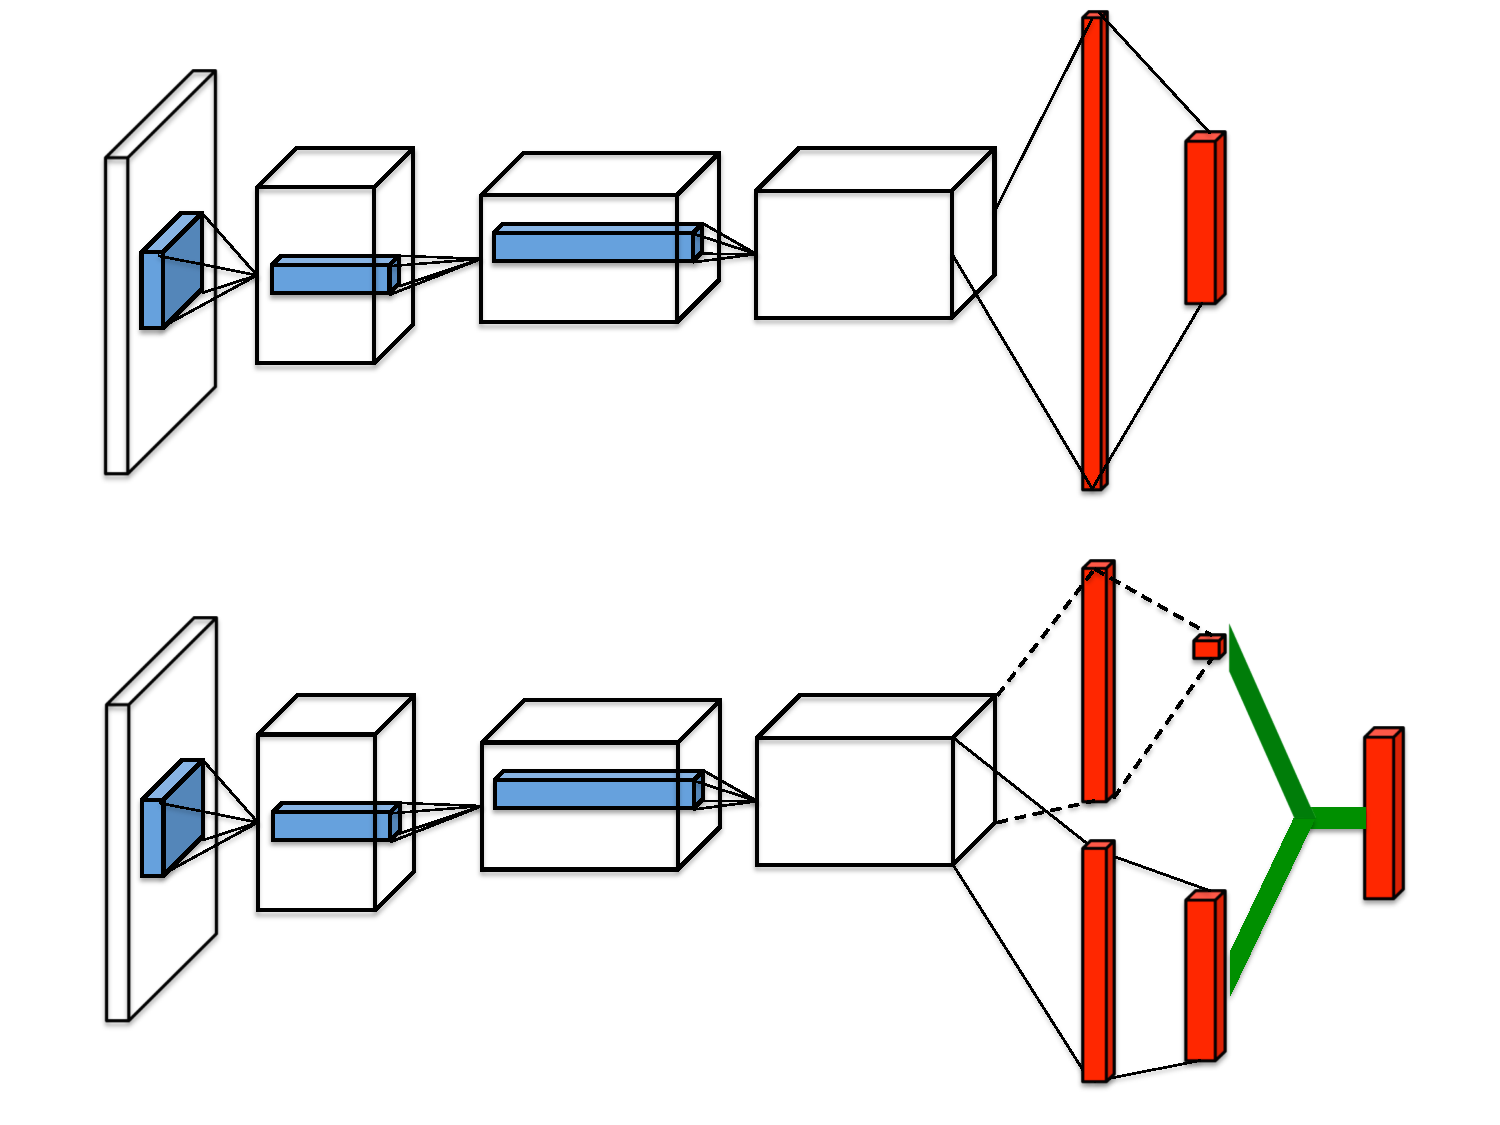
\includegraphics[width=0.95\linewidth]{fig/ddqn.pdf}
\caption[Dueling Network Architecture]{The dueling network architecture \cite{wang15_duelin_networ_archit_deep_reinf_learn} \label{fig-model-dueling}}
\end{figure}


Our agent uses the dueling DDQN algorithm with a standard neural network
architecture, similar to the one depicted in Figure \ref{fig-ann}. It consist of
four input nodes (number of states), three fully-connected hidden layers with
ReLU activation functions, and a linear output layer with two nodes (number of
actions). Further, an \(\epsilon\)-greedy policy with a linear decreasing
exploration rate was used. The RL agent was implemented with the neural networks
API Keras\footnote{\url{https://www.keras.io}}\textsuperscript{,}\,\footnote{\url{https://github.com/keras-rl/keras-rl}}, which is a high-level abstraction layer of TensorFlow.
TensorFlow is the de-facto standard for robust and scalable machine learning in
industry and research \cite{abadi16_tensor}. Further, we used the shared research
environment Google Colaboratory\footnote{\url{https://colab.research.google.com}} to train and evaluate the agent. It offers
free access to computing resources that are optimized for training machine
learning models. More specifically, it provides a NVIDIA Tesla K80 GPU, with
2880 \(\times\) 2 CUDA cores and 12GB GDDR5 VRAM . Additionally, the environment
is equipped with a Intel(R) Xeon(R) CPU @ 2.30GHz (1 core, 2 threads), and over
12GB available memory. Google Colaboratory can be used up to 12 hours of
consecutive training.

\clearpage

\section{Simulation Platform: FleetSim}
\label{sec:org7099106}
\begin{itemize}
\item Simulation Platform to allow evaluating the performance of intelligent agents
in smart charging/balancing the grid of EV fleets. Allows to test out bidding
strategies and control mechanisms in a realistic EV fleet setting.
\item Real life comparison graph: 10\%.
\end{itemize}
\subsection{Event-based Simulation}
\label{sec:org1b17616}
\begin{itemize}
\item Not only t+1
\item Event e.g. denying rental, charge/little charge/no-charge has effects for the
whole simulation
\item Simpy
\item Python
\end{itemize}
\subsection{Architecture / Components}
\label{sec:org9cda77e}

\subsection{Modular Expandability}
\label{sec:org6731b15}
\begin{itemize}
\item Plug-in different Market designs
\item Use different real-world data
\item Change Fleet parameters
\item Develop new strategy
\item
\end{itemize}
\section{Results}
\label{sec:org4ef4ff0}
\subsection{Simulation Settings}
\label{sec:orgc4e9e95}
\begin{itemize}
\item Results heavily dependent on industry charging price, since on average the
balancing prices are 50\% cheaper, and intraday 30\% cheaper.
\item BMWi. (n.d.). Prices of electricity for the industry in Germany from 2008 to
2017 (in euro cents per kilowatt hour). In Statista - The Statistics Portal.
Retrieved March 18, 2019, from
\url{https://www.statista.com/statistics/595803/electricity-industry-price-germany/}.
\end{itemize}
\subsection{FleetRL}
\label{sec:org1d60e77}
\begin{itemize}
\item long-delayed rewards make RL hard (!?)
\item Compare RL Algos eg. Q-learning vs DDQN --> deep learning makes difference in
practice for complex system
\item How much could have been used as VPP optimally/perfect information? Similar matrix to Kahlen, or even plot?
\end{itemize}
\subsection{Sensitivity Analysis}
\label{sec:orga9a2bc0}
\begin{itemize}
\item Prediction Accuracy
\end{itemize}

\begin{itemize}
\item Charging infrastructure
\end{itemize}
\section{Conclusion}
\label{sec:org8ec2f28}
\subsection{Contribution}
\label{sec:org58c860e}
\begin{itemize}
\item Compare to most simular studies:
\end{itemize}
\cite{kahlen18_elect_vehic_virtual_power_plant_dilem,vandael15_reinf_learn_heuris_ev_fleet} etc..
\begin{itemize}
\item Business model for EV fleet owners with better results than previous studies
\item Environmental impact by providing balancing power
\item Decision Support System for controlled EV charging from multiple markets
\item RL Algorithm that is designed to work in previously unknown environments and
thus suited to deploy in real life settings of all kinds of EV fleets in all
kinds of cities. E.g. scooters also?
\item Event-based Simulation Platform to evaluate bidding strategies and RL agents,
facilitate research
\end{itemize}

\subsection{Limitations}
\label{sec:orgda72435}
\begin{itemize}
\item Model:
\begin{itemize}
\item Bidding Mechanism: one week ahead, always accepted
\item Policy \& Regulation: EVs not allowed to provide balancing power, minimum
bidding quantities 1MW.
\item Markets: Fleet is a price-taker, what about larger fleets? Simulate market influence
\end{itemize}
\item RL: See \cite{vazquez-canteli19_reinf_learn_deman_respon} conclusion for
limitations.
\end{itemize}
\subsection{Future Research}
\label{sec:org3341dfb}
\begin{itemize}
\item Model: Current market design, i.e. daily w/ 4h slots. German "Mischpreisverfahren"
\item RL: Long-delayed rewards, different reward structure, memory based
\end{itemize}

\clearpage
\bibliography{bibliography/references}
\bibliographystyle{apacite}
\end{document}
